\chapter{Introduction}
\label{chap:intro}

\section{Motivation}

This paper aims to study benchmark datasets for human disease genes, exploiting the link between the human genome and diseases. By analyzing vast genetic data obtained from various sources e.g  DisGeNET, HuGE Navigator the research seeks to help in developing new treatments and fostering improved patient care. The standardized datasets will serve as a foundation for comprehensive investigations in this vast research field and promote collaboration among researchers. The collection of the datasets will provide significant insights to the researchers. Ultimately, this work holds promise for advancing disease management and personalized medicine, benefiting society as a whole.

\section{Problem Statement}

The problem of finding benchmark datasets for human disease genes revolves around the scarcity of readily available and standardized datasets. Existing resources such as OMIM and DisGeNet contain datasets that often lack standardization, hindering their immediate use for benchmarking purposes. The credibility of datasets claiming to be benchmarked needs verification to ensure their reliability. The fragmented distribution of benchmark datasets across various platforms further complicates the process of locating relevant information. Addressing this problem requires the development and evaluation of benchmark datasets to provide researchers with reliable and accessible resources for their studies. 

\section{Objective}

Our thesis aims to study benchmark datasets for Human disease genes which involves analyzing large and complex datasets including genetic and clinical data. The objective is to compare the performance of the methods and tools used to create and evaluate the benchmark  datasets in the state of art literature. 

\section{Document Summary}

Here, the overall structure of our thesis report is briefly described. The current introduction chapter contains our motivation, the problem definition and main goals. The remaining chapters have been organized as follows:

Chapter 2: This chapter includes a background study on the problem domain and discussion on relevant papers of studies previously conducted.

Chapter 3: This chapter includes discussion of the benchmarking process.

Chapter 4: In this chapter, each element of our proposed method is elaborated in detail.

Chapter 5: This chapter provides discussion about future work and conclusion.

\chapter{Background \& Literature Review}


\section{Genomics}


 

\subsection{Gene}

A gene is a basic unit of heredity that carries the instructions for making a specific protein. A gene is made up of DNA, which is a molecule that contains the genetic code. The genetic code is a set of instructions that tells cells how to make proteins. Proteins are the building blocks of cells and they carry out many important functions in the body. Genes are passed down from parents to offspring, and they determine many of our physical traits.

 

\subsection{Gene Disease Association}

Gene-disease associations\cite{1} serve as foundational pillars upon which advancements in clinical diagnostic methodologies can be built. By identifying the specific genetic signatures associated with particular diseases, researchers can develop targeted diagnostic tests that enable early detection, accurate diagnosis, and risk stratification. This information empowers clinicians to tailor treatment plans to individual patients, optimizing therapeutic efficacy and minimizing adverse effects.


 

 

\section{Human Gene-Disease Datasets}


\subsection{Raw Dataset}

The raw dataset would encompass the unrefined, original data gathered for the study. This data collection process might entail extracting information on gene-disease associations, genetic variations, and other pertinent attributes that are crucial for understanding the genetic underpinnings of human diseases.

Raw datasets often have missing information, either because of mistakes when collecting the data, or because the information was not available or not recorded completely. If this missing information is not fixed, it can make the analyses less complete and might lead to unfair results. Raw datasets might also have mistakes, like wrong numbers or different ways of collecting the data. These mistakes can make the analyses less accurate and make it harder to get good results. 

Genetic data are scattered across different domains and databases (i.e. OMIM\cite{2}, CTD\cite{3}, DisGeNET\cite{4}, ClinVar\cite{5}, Uniprot\cite{6}, Orphanet\cite{7}, GAD\cite{8}, GWAS Catalogue\cite{9}, dbGaP\cite{10}).The identification and prioritization of the relevant information from that scattered and vast quantity of data is often a challenging task for the end user. Another Difficulty that arises is, the research on the domain of genomics is that the data is only available as free text in scientific publications and this data is not compatible for computational analysis. Working with these types of data is not suitable and a slow process.  

\subsection{Tools Employed for Genomic Data Extraction}

Creating benchmark datasets uses different sequencing technologies\cite{11}. This sequencing technologies benefited in the development of genomic, transcriptomic, and epigenomic studies. Gene sequencing technologies focus on decoding the genetic information encoded in DNA and RNA. These sequencing technologies gather a large amount of data but the text mining tools play a crucial role in extracting valuable information from the vast amount of scientific literature and textual data associated with genomics. In recent years, the rapid progress of artificial intelligence has significantly advanced natural language processing (NLP), merging linguistic principles, computer science, and mathematics \cite{12}\cite{13}\cite{14}. NLP facilitates human-computer communication. Text classification within NLP is a fundamental task, systematically assigning a given text to predefined categories based on specific characteristics\cite{15}. The process involves three key steps: text preprocessing, vector representation extraction, and training a classifier for effective categorization\cite{16}. Text classification is divided into single-label and multi label types, depending on whether each text is associated with one or more categories\cite{17}\cite{18}\cite{19}. Single-label assigns one category per text, while multilabel allows for multiple category assignments.

In the past, most efforts in text mining of relationships have been devoted to the identification of interactions between proteins, both due to the availability of corpora and the push driven by specific text mining challenges\cite{20}. But In recent years, many text mining tools have been developed for the purpose of classification genomics data. BeFree is a text mining tool used to recognize  biomedical entities that identifies genes, diseases, and chemicals from scientific texts using rule-based and dictionary-based approaches. By exploiting morpho-syntactic information of the text, BeFree is able to identify gene-disease, drug-disease and drug-target associations with state-of-the-art performance. Named Entity Recognition (NER) is a crucial task in natural language processing (NLP) that involves identifying and classifying entities. NER operates by recognizing and categorizing specific terms or phrases that represent entities, contributing to the overall comprehension of textual data. The goal of NER is to identify, within a collection of text, all of the instances of a name for a specific type of thing: for example, all of the drug names within a collection of journal articles, or all of the gene names and symbols within a collection of MEDLINE abstracts.\cite{21}

BERT\cite{22} is a contextualized word representation model that is based on a masked language model and pre-trained using bidirectional transformers. BERT to classify genetic mutations based on text evidence from an annotated database\cite{23}. BioBERT (Bidirectional Encoder Representations from Transformers for Biomedical Text Mining), is a domain-specific language representation model pre-trained on large-scale biomedical corpora. BioBERT largely outperforms BERT and previous state-of-the-art models in a variety of biomedical text mining tasks when pre-trained on biomedical corpora.\cite{24}

There are other tools available in the literature i.e. PubTator\cite{25}, MetaMap\cite{26}.

These tools play a vital role in knowledge discovery, offering efficient and speedy extraction of relevant information from diverse textual sources. The integration of heterogeneous data types, including genetic and clinical information, benefits from automated extraction processes. Text mining facilitates literature reviews and summarization, enabling researchers to quickly grasp key insights and trends. Overall, these tools are indispensable for navigating and interpreting the vast landscape of genomics literature, accelerating knowledge discovery and advancing genomic research.

BeFree is a text mining tool designed to identify biomedical entities such as genes, diseases, and chemicals in scientific literature.

 
\subsection{DisGeNet}

The DisGeNET which was first released on September, 2010 a database which integrates information of human gene-disease associations (GDAs) and variant-disease associations (VDAs) from various repositories including Mendelian, complex and environmental diseases.DisGeNET integrates data from expert curated repositories, GWAS catalogues, animal models and the scientific literature. These data are complemented with information extracted from the scientific literature using NLP-based text-mining tools. A distinctive feature of DisGeNET is its unique collection of GDAs and VDAs extracted by text mining the scientific literature.\cite{27}

DisGeNET seamlessly integrates meticulously curated databases with text-mined data, encompassing a comprehensive spectrum of information on both Mendelian and complex diseases. Accessible through multiple platforms, including a web interface, a Cytoscape plugin, and as a Semantic Web resource, \textit{scripts in several programming languages and an R package,} DisGeNET stands as an open-access repository, representing one of the most extensive and comprehensive collections of associations between human genes and diseases.Here, the data were combined from curated datasets called “OMIM, UNIPROT, PHARMGKB, CTD, CURATED”. As a result, DisGeNET is a coherent tool for easy analysis and interpretation of human gene–disease networks.


\begin{figure}[!h]
    \centering
    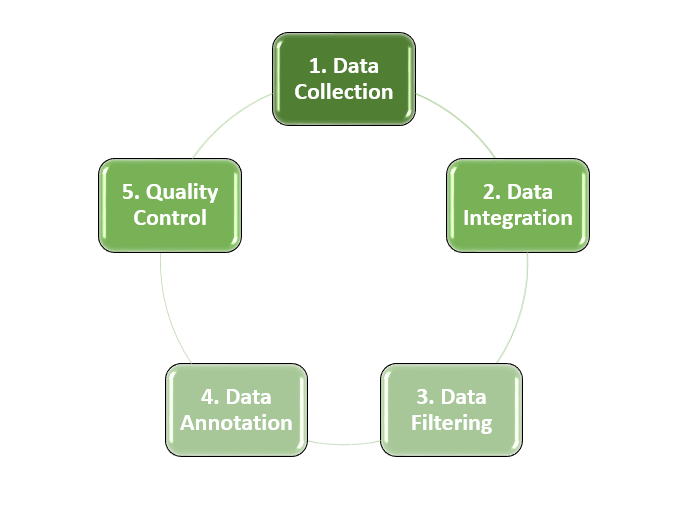
\includegraphics[width=0.75\linewidth]{DisGeNET Flow.PNG}
    \caption{DisGeNET Flow Diagram}
    \label{fig:DisGeNETl}
\end{figure}

In DisGeNet we can see the continuous update, As DisGeNET 4.0 (June, 2016)\cite{27} contained 429 036 gene-disease associations (GDAs), linking 17 381 genes to 15 093 diseases which gradually improved in 08 January 2020. In that time, the database(v6.0)\cite{28} contained 628 685 gene-disease associations (GDAs), involving 17 549 genes and 24 166 diseases, and 210 498 variant-disease associations (VDAs), including 117 337 variants and 10 358 diseases. The latest updated of DisGeNET is shown below in the table:

\textbf{The current version of DisGeNET (v7.0):}
\begin{table}
	\centering
	\begin{tabularx}{\textwidth}{|X|X|X|X|}
		\hline
		\textbf{Category} & \textbf{Clinical Concepts} & \textbf{Associated Genes} & \textbf{Associated Variants} \\
		\hline
		Disease & 21838 & 20163 & 139004 \\
		Disease Group & 962 & 15474 & 22477 \\
		Phenotype & 7493 & 16854 & 62686 \\
		\hline
	\end{tabularx}
	\caption{The current version of DisGeNET (v7.0)}
\end{table}

 

\subsection{OMIM}
{An Online Catalog of Human Genes and Genetic Disorders,OMIM was first introduced in the 60s. Dr. McKusick, the initiator of the Online Mendelian Inheritance in Man (OMIM)\cite{29} database, started collecting information about genes and their association to diseases first as a book and later as a database. OMIM has become a highly popular source in medical genetics.OMIM entries have a structured free-text format between genes and genetic phenotypes that provides complex relationships in an efficient manner.\cite{30}}

OMIM is a well-established database with a long history of expert curation, making it a reliable source for accurate and comprehensive information on Mendelian disorders. It also provides detailed literature curation for each gene-disease association, offering in-depth supporting evidence. OMIM is recommended for research focused on Mendelian disorders and requiring in-depth literature curation.  \newline

\begin{figure}[!h]
    \centering
    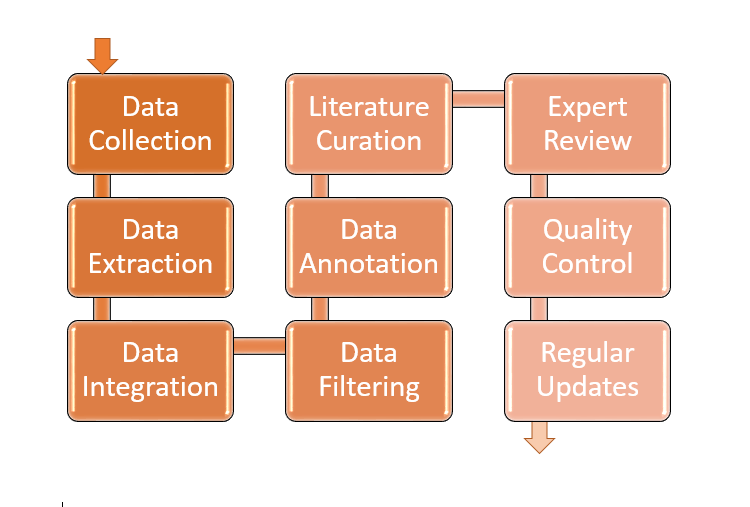
\includegraphics[width=0.7\linewidth]{OMIM FLOW.PNG}
    \caption{OMIM Work Process}
    \label{fig:OMIM Flow Diagram}
\end{figure}
\vspace{1cm}
\textbf{Other available Databases:}
\newline The Comparative Toxicogenomics Database (CTD) that provides information about chemicals and genes, and their effect in human health and disease.\cite{3}
UniProt, a repository centred on protein sequence and function, that also include disease annotations from OMIM, and from expert curation of the scientific literature.\cite{6} 
ClinVar: a public archive of relationships between human variants and phenotypes, including diseases.


\begin{table}
    \resizebox*{!}{1 in}{%
        \parbox{1 in}{%
            \begin{tabular}{|c|c|c|} \hline 
                \textbf{Feature} & \textbf{OMIM} & \textbf{DisGeNET}\\ \hline 
                Research Focus & Mendelian disorders & Broad range of gene-disease associations\\ \hline 
                Data Quality & Expert curation & Automated and manual curation\\ \hline 
                Data Coverage & Limited to Mendelian disorders & Broader coverage, including complex and non-Mendelian disorders\\ \hline 
                Data Updates & Regular, but may lag behind DisGeNET & Very frequent updates\\ \hline 
                Genomic Data Integration & Limited & Integrated with genetic variants and expression profiles\\ \hline 
                Community Involvement & Limited & Open-source, fostering community contributions\\ \hline
            \end{tabular}
        }% <-- Closing brace for \parbox
    }% <-- Closing brace for \resizebox
    \caption{Difference between OMIM and DisGeNET}
    \label{tab:my_label}
\end{table}

\begin{table}
		\begin{tabularx}{\textwidth}{|X|X|X|X|X|X|X|}
			\hline 
			\textbf{Name} & \textbf{URL} & \textbf{Scope} & \textbf{Organism} & \textbf{Current Statistics} & \textbf{Original Reference} & \textbf{Current Reference} \\
			\hline 
			DisGeNET & \url{http://disgenet.org} & Gene-disease, and variant-disease associations & Human & 1,134,942 associations, between 21,671 genes and 30,170 diseases & 2010 \cite{31} & \cite{4} \\
			Comparative Toxicogenomics Database(CTD) & \url{http://ctdbase.org/} & Chemicals, genes, and disease associations & Human and animal models & 46,589 SNPs & 2003 \cite{32} & \cite{3} \\
			Online Mendelian Inheritance in Man(OMIM) & \url{http://www.omim.org} & Mendelian diseases and their genes & Human & 1,127,498 associations between & 1998 \cite{33} & \cite{2} \\
			Genetic Association Database(GAD) & \url{http://geneticassociationdb.nih.gov/} & Genes, variants, and complex diseases and traits & Human & 20,027 genes and 1,504 diseases & 2004 \cite{8} & (8) \\
			UniProt Knowledgebase & \url{http://www.uniprot.org/} & Proteins & Human & 121,512 associations between 29,596 diseases and 20,790 & 2004 \cite{34} & \cite{6} \\
			The NHGRI-EBI Catalog of published GWAS (GWAS Catalog) & \url{http://www.ebi.ac.uk/gwas/} & GWAS studies & Human & genes & 2009 (35) & \cite{9} \\
			\hline
		\end{tabularx}
		\caption{\textbf{Comparative Study Between Different Standard Datasets}}
		\label{tab:my_label}
\end{table}

\newpage


	

\section{Machine Learning}
\subsection{Types of Machine Learning Models}
There are four main types of machine learning models:

\begin{enumerate}
    \item \textbf{Supervised learning}: In supervised learning, the algorithm is trained on a labeled dataset, where each data point has a corresponding label or output value. The algorithm learns to map the input data to the desired output values. Supervised learning algorithms can be used for both classification and regression tasks.

\begin{itemize}
        \item Classification: Classification algorithms are used to predict a discrete category or label for each data point. Examples of classification algorithms include logistic regression, support vector machines (SVMs), and decision trees.

        \item Regression: Regression algorithms are used to predict a continuous numerical value for each data point. Examples of regression algorithms include linear regression, polynomial regression, and neural networks.

\end{itemize}

    \item \textbf{Unsupervised learning}: In unsupervised learning, the algorithm is trained on a dataset without labels. The algorithm learns to identify patterns and relationships in the data without any prior knowledge of the data's structure or meaning. Unsupervised learning algorithms can be used for clustering, dimensionality reduction, and anomaly detection tasks.

\begin{itemize}
        \item Clustering: Clustering algorithms are used to group similar data points together. Examples of clustering algorithms include k-means clustering, hierarchical clustering, and density-based spatial clustering of applications with noise (DBSCAN).

        \item Dimensionality reduction: Dimensionality reduction algorithms are used to reduce the number of features or variables in a dataset. This can be useful for simplifying data analysis and improving the performance of machine learning algorithms. Examples of dimensionality reduction algorithms include principal component analysis (PCA) and t-distributed stochastic neighbor embedding (t-SNE).

        \item Anomaly detection: Anomaly detection algorithms are used to identify data points that are significantly different from the rest of the data. This can be useful for detecting fraud, detecting errors in data, or identifying new and unusual patterns in data. Examples of anomaly detection algorithms include one-class SVMs, isolation forests, and outlier detection based on local outlier factor (LOF).

\end{itemize}

    \item \textbf{Reinforcement learning}: In reinforcement learning, the algorithm learns to interact with an environment by taking actions and receiving rewards or penalties. The algorithm learns to choose actions that maximize the cumulative reward over time. Reinforcement learning is often used in robotics, game playing, and other applications where the goal is to achieve a long-term objective.

    \item Semi-supervised learning: Semi-supervised learning is a hybrid approach that combines supervised and unsupervised learning. The algorithm is trained on a dataset that includes both labeled and unlabeled data. The algorithm learns from the labeled data to identify patterns and relationships, and then uses those patterns to label the unlabeled data. Semi-supervised learning is often used when there is a limited amount of labeled data available.
\end{enumerate}
 
\subsection{Machine Learning Models for Gene Disease Association}

Here, are some of the best machine learning models to find the best accuracy for a gene-disease associated benchmark dataset:

\textbf{1. Decision Tree (DT):}

A decision tree is a non-parametric supervised learning method used for both classification and regression tasks. It is a hierarchical, tree-like structure that consists of a root node, internal nodes, and leaf nodes. The root node represents the entire dataset, while the internal nodes represent the features or attributes of the data. The leaf nodes represent the predicted classes or values for the data points.

\textbf{How Decision Trees Work:}

Decision trees work by recursively partitioning the data into smaller subsets based on the values of the features. At each node, the algorithm selects the feature that best separates the data into two subsets. This process of splitting the data is repeated until each subset is pure, meaning that all data points in the subset belong to the same class.

\textbf{Advantages of Decision Trees:}

\begin{itemize}
    \item Interpretability: Decision trees are highly interpretable, as the decision path from the root node to the leaf node represents the decision-making process. This makes it easy to understand how the model makes its predictions.

    \item Robustness to outliers: Decision trees are relatively robust to outliers, as they are not sensitive to changes in individual data points.

    \item Non-parametric: Decision trees are non-parametric, meaning that they do not make any assumptions about the underlying distribution of the data.

\end{itemize}
\textbf{Disadvantages of Decision Trees:}

\begin{itemize}
    \item Overfitting: Decision trees can overfit the data, meaning that they memorize the training data and do not generalize well to new data. This can be mitigated by using techniques such as pruning and regularization.

    \item High dimensionality: Decision trees can become very large and complex when dealing with high-dimensional data. This can make them difficult to interpret and computationally expensive to train.

\end{itemize}
\textbf{Applications of Decision Trees:}

Decision trees are used in a wide variety of applications, including:

\begin{itemize}
    \item Medical diagnosis: Decision trees can be used to diagnose diseases based on patient symptoms and test results.

    \item Fraud detection: Decision trees can be used to detect fraudulent transactions based on spending patterns and other factors.

    \item Customer segmentation: Decision trees can be used to segment customers based on their demographics, purchase history, and other factors.

    \item Risk assessment: Decision trees can be used to assess the risk of events such as loan defaults or customer churn.

\end{itemize}

\textbf{2. Support Vector Machines (SVMs):}

SVMs are another powerful classification algorithm that can be used for gene-disease association prediction. SVMs work by finding the optimal hyperplane that separates the two classes (genes associated with disease and genes not associated with disease) with the largest margin. SVMs are generally more computationally expensive to train than logistic regression, but they can achieve higher predictive accuracy in some cases.

Support Vector Machines (SVMs) are supervised learning algorithms used for classification and regression tasks. They are particularly well-suited for classification tasks, where the goal is to predict a discrete category for each data point. SVMs are known for their ability to handle high-dimensional data and their robustness to outliers.

\textbf{How SVMs Work:}

SVMs work by finding a hyperplane that separates the data points into two classes with the largest margin. The margin is the distance between the hyperplane and the closest data points from each class. SVMs find the hyperplane that maximizes the margin, which generally leads to a better classification model.

\textbf{Advantages of SVMs:}

\begin{itemize}
    \item High-dimensional data: SVMs can handle high-dimensional data without overfitting.

    \item Robustness to outliers: SVMs are relatively robust to outliers, as they are not sensitive to changes in individual data points.

    \item Interpretability: SVMs can be made interpretable by using kernel methods, such as the linear kernel or the polynomial kernel.

\end{itemize}
\textbf{Disadvantages of SVMs:}

\begin{itemize}
    \item Computational complexity: SVMs can be computationally expensive to train, especially when dealing with large datasets.

    \item Parameter tuning: SVMs require careful parameter tuning, such as the choice of the kernel function and the regularization parameter.

\end{itemize}
\textbf{Applications of SVMs:}

SVMs are used in a wide variety of applications, including:

\begin{itemize}
    \item Image classification: SVMs are used to classify images, such as handwritten digits or human faces.

    \item Text classification: SVMs are used to classify text documents, such as spam email or news articles.

    \item Bioinformatics: SVMs are used to predict gene function or protein structure.

    \item Anomaly detection: SVMs are used to detect anomalies or outliers in data.

\end{itemize}
Overall, SVMs are powerful and versatile machine learning algorithms that are well-suited for a wide variety of tasks. They are particularly well-suited for classification tasks, where the goal is to predict a discrete category for each data point.

\textbf{3. Random Forests:}

Random forests are an ensemble learning method that combines multiple decision trees to improve predictive performance. Random forests are robust to outliers and can handle high-dimensional data, making them well-suited for gene-disease association prediction.

Random Forest (RF) is an ensemble learning method used for both classification and regression tasks. It is a powerful and versatile algorithm that can handle high-dimensional data and is relatively robust to outliers. RF is based on the concept of bagging, which involves creating multiple decision trees and combining their predictions to improve overall accuracy.

\textbf{How RF Works:}

\begin{enumerate}
    \item Bagging: RF creates a set of decision trees by sampling the training data with replacement. This means that some data points may be selected multiple times, while others may not be selected at all.

    \item Feature Randomness: At each node in each decision tree, RF randomly selects a subset of features to consider for splitting. This helps to reduce the correlation between the trees and prevent overfitting.

    \item Voting: RF combines the predictions of the individual decision trees by majority voting for classification tasks or by averaging for regression tasks.

\end{enumerate}

\textbf{Advantages of RF}:

\begin{itemize}
    \item High accuracy: RF can achieve high accuracy on a wide variety of tasks.

    \item Robustness to outliers: RF is relatively robust to outliers, as it is not sensitive to changes in individual data points.

    \item Feature importance: RF can provide information about the relative importance of different features in the data.

    \item No feature scaling: RF does not require feature scaling, which can make it easier to use with raw data.

\end{itemize}
\textbf{Disadvantages of RF:}

\begin{itemize}
    \item Interpretability: RF can be difficult to interpret, as the individual decision trees can be complex.

    \item Computational complexity: RF can be computationally expensive to train, especially when dealing with large datasets.

    \item Hyperparameter tuning: RF requires careful hyperparameter tuning, such as the number of trees and the number of features to consider at each split.

\end{itemize}

\textbf{Applications of RF:}

RF is used in a wide variety of applications, including:

\begin{itemize}
    \item Fraud detection: RF can be used to detect fraudulent transactions based on spending patterns and other factors.

    \item Customer segmentation: RF can be used to segment customers based on their demographics, purchase history, and other factors.

    \item Risk assessment: RF can be used to assess the risk of events such as loan defaults or customer churn.

    \item Medical diagnosis: RF can be used to diagnose diseases based on patient symptoms and test results.

\end{itemize}
Overall, RF is a powerful and versatile machine learning algorithm that is well-suited for a wide variety of tasks. It is particularly well-suited for tasks where accuracy and robustness are important.

\textbf{4. Neural Networks:}

Neural networks are a powerful class of machine learning models that can be used for both classification and regression tasks. Neural networks are inspired by the structure of the human brain and can learn complex relationships between input and output data. Neural networks can be very effective for gene-disease association prediction, but they can also be computationally expensive to train and require a large amount of training data.

Neural Networks (NN) are a type of machine learning algorithm inspired by the structure and function of the human brain. They are composed of interconnected nodes or "neurons" that communicate with each other through weighted connections. NN are capable of learning from data and making predictions or decisions without explicit programming.

\textbf{Structure of Neural Networks:}

NN are typically organized in layers:

\begin{enumerate}
    \item Input Layer: The input layer receives the raw data to be processed.

    \item Hidden Layers: Hidden layers perform the computations and transformations of the data. There can be multiple hidden layers, each with its own set of neurons.

    \item Output Layer: The output layer produces the final predictions or decisions.

\end{enumerate}
Learning in Neural Networks:

NN learns through a process called training. During training, the NN is presented with a set of training data, consisting of input data and corresponding desired output values. The NN adjusts the weights of the connections between neurons to minimize the error between its predictions and the desired output values. This process is repeated until the NN's predictions are sufficiently accurate.

\textbf{Types of Neural Networks:}

There are various types of NN, each with its own strengths and applications:

\begin{enumerate}
    \item Perceptrons: The simplest form of NN, capable of linear classification tasks.

    \item Multilayer Perceptrons (MLPs): An extension of perceptrons, allowing for nonlinear relationships in the data.

    \item Convolutional Neural Networks (CNNs): Particularly effective for image recognition and processing.

    \item Recurrent Neural Networks (RNNs): Designed to handle sequential data, such as text or time series data.

\end{enumerate}
Applications of Neural Networks:

\textbf{NN have revolutionized various fields, including:}

\begin{enumerate}
    \item Image Recognition: NN are used to identify objects, faces, and scenes in images and videos.

    \item Natural Language Processing (NLP): NN are used for tasks like machine translation, sentiment analysis, and text summarization.

    \item Speech Recognition: NN are used to convert spoken language into text.

    \item Anomaly Detection: NN can identify unusual patterns or outliers in data.

    \item Recommender Systems: NN are used to suggest products, movies, or music based on user preferences.

    \item Predictive Analytics: NN can predict future outcomes based on historical data.

    \item Medical Diagnosis: NN can assist in diagnosing diseases based on patient symptoms and medical images.

\end{enumerate}
Neural Networks are a powerful and versatile tool in machine learning, capable of tackling complex tasks and making accurate predictions. Their ability to learn from data and adapt to new information makes them increasingly valuable in various domains.

As you can see, all four models have their own strengths and weaknesses. The best model for a particular task will depend on the specific requirements of that task.

Here is a table summarizing the key differences between the four models:
\newpage
 \begin{table}
    \centering
    \resizebox{\textwidth}{!}{%
        \begin{tabular}{|c|c|c|c|c|} \hline 
            \textbf{Feature}
            & \textbf{Logistic Regression}
            & \textbf{SVM}
            & \textbf{Random Forest}
            & \textbf{Neural Networks} \\ \hline 
            Classification
            & Binary
            & Binary and multi-class
            & Binary and multi-class
            & Binary and multi-class \\ \hline 
            Regression
            & No
            & Yes
            & Yes
            & Yes \\ \hline 
            Interpretability
            & High
            & High
            & Low
            & Low \\ \hline 
            Computational complexity
            & Low
            & Medium
            & High
            & High \\ \hline 
            Robustness to outliers
            & Low
            & High
            & High
            & High \\ \hline 
            Feature scaling
            & No
            & No
            & No
            & Yes \\ \hline
        \end{tabular}
    }
    \caption{Differences Between The Four Models}
    \label{tab:model_differences}
\end{table}
	\begin{table}
		\centering
		\small  % Smaller font size
		\resizebox{\textwidth}{!}{%
			\begin{tabular}{|c|p{3.5cm}|p{4cm}|p{4cm}|} \hline 
				\textbf{Model}
				& \textbf{Description}
				& \textbf{Advantages}
				& \textbf{Disadvantages} \\ \hline 
				Support Vector Machines (SVM)
				& A supervised learning algorithm used for classification and regression tasks.
				& High-dimensional data, robustness to outliers, interpretability
				& Computational complexity, parameter tuning \\ \hline 
				Random Forest (RF)
				& An ensemble learning method used for both classification and regression tasks.
				& High accuracy, robustness to outliers, feature importance, no feature scaling
				& Interpretability, computational complexity, hyperparameter tuning \\ \hline 
				Neural Networks (NN)
				& A type of machine learning algorithm inspired by the structure and function of the human brain.
				& High accuracy, ability to learn from data, adaptability
				& Computational complexity, interpretability, hyperparameter tuning \\ \hline 
				Logistic Regression
				& A statistical model used for binary classification tasks.
				& Interpretability, simplicity, computational efficiency
				& Not suitable for multi-class classification tasks \\ \hline
			\end{tabular}
		}
		\caption{Summary of the Four Models}
		\label{tab:model_summary}
	\end{table}
\newpage
\textbf{ Summarize up:}
\begin{itemize}
    \item SVM, RF, NN are all powerful machine learning algorithms that can be used for a variety of tasks.
    \item SVM is well-suited for high-dimensional data and is robust to outliers.
    \item RF is known for its high accuracy and ability to handle complex relationships in data.
    \item NN are capable of learning from data and making accurate predictions without explicit programming.
    \item Logistic Regression is a simple and interpretable algorithm that is well-suited for binary classification tasks.
\end{itemize}
The best machine learning model for your gene-disease association benchmark dataset will depend on the specific characteristics of your data, such as the size of the dataset, the number of genes and diseases, and the quality of the data. It is often a good idea to try several different models and compare their performance on a validation set to find the best model for your task.

 

\section{Study of Existing Papers}
\subsection{Benchmark data set for breast cancer associated genes\cite{35}} 
The goal of the study was to explore the association of breast cancer genes by classifying them into different association classes: positive, negative, and neutral. The researchers obtained raw data from the HuGE Literature Finder via\href{https://phgkb.cdc.gov/PHGKB/startPagePubLit.action}{ https://phgkb.cdc.gov/PHGKB/startPagePubLit.action}, which provided PubMed IDs related to breast cancer. To extract abstract text data from these PubMed IDs, the researchers used EDirect, a tool developed by NCBI for data retrieval from PubMed.

A total of 12,565 records were processed to eliminate anomalies, duplicate entries, and redundancy. The researchers successfully extracted 12,565 reference sentences containing at least one disease and gene term from 7,073 abstracts. The method employed for processing the raw data was double-fold cross-validation, which helped discard false predictions and generate a processed file used to calculate the weight of individual gene association classes.

The researchers used benchmark gene reference data for breast cancer, which can be found at\href{https://data.mendeley.com/datasets/xdkvk75ns7/2}{ https://data.mendeley.com/datasets/xdkvk75ns7/2}.

In summary, the study focused on the association of breast cancer genes, utilizing a robust methodology involving data from the HuGE Literature Finder, EDirect, and a double-fold cross-validation process. The benchmark gene reference data served as a comparison for the classification of gene association classes.

 
\subsection{Benchmarking network propagation methods for disease gene identification\cite{36}}
The article focuses on evaluating and comparing various computational techniques for predicting or prioritizing genes associated with specific diseases. The code and datasets supporting the conclusions can be found on the GitHub repository\href{https://github.com/b2slab/genedise}{ https://github.com/b2slab/genedise}.

The benchmarking process involves assessing and comparing the performance of different network propagation methods to identify the most effective one for disease gene identification. The key steps in the benchmarking process include Data Preparation, Method Selection, Cross-validation, Comparison, Statistical Analysis, and Visualization.

The primary objective of the study was to identify genes that could be targeted by drugs for treating common diseases. The researchers utilized data from the OpenTargets database, which provides information about genes and diseases.

The study employed 12 different computer algorithms proficient in analyzing biological networks. These algorithms were tested on data related to 22 common diseases. Two types of data were considered: genetic information related to diseases and data about how genes interact with each other and with proteins.

To ensure the reliability of their results, the researchers used cross-validation, a special testing method for algorithms. The majority of the project was coded in R, with some Matlab code required to incorporate state-of-the-art approaches.

In summary, the article presents a comprehensive evaluation and comparison of computational techniques for predicting disease-associated genes. The study involves the use of diverse algorithms, data types, and the OpenTargets database, and the results are supported by thorough cross-validation.

 
\subsection{Genomic variant benchmark: if you cannot measure it, you cannot improve it\cite{11} }
Genome variant benchmark datasets are important for assessing variant callers. They help to improve variant detection methods. Benchmark datasets should include information about genomic regions with variants.

Creating benchmark datasets uses different sequencing technologies. These include long-reads, short-reads, and linked-reads. It is hard to get perfect accuracy and sensitivity, but the processes of sequencing, read alignment, genome assembly, and variant calling help to make better pipelines and technologies.

Benchmark dataset curation uses different sequencing technologies to overcome limitations and errors. Groups like the Genome in a Bottle Consortium (GIAB) and Platinum Genome are working to make or improve benchmark datasets.

The CMRGs benchmark dataset looks at challenging genes that were not fully studied in other benchmark datasets. These Clinically Meaningful Reference Genes (CMRGs) have been studied a lot and are linked to one or more diseases.

Short-read technologies, like Illumina's exome sequencing, are common because they are cheap and accurate. But they do have limitations. Long-read sequencing technology may be able to find structural variants (SVs) that cause diseases that short-read sequencing misses. HiFi long-reads are being used to make a group of genes from different databases. This shows that scientists are working to fix problems and improve benchmark datasets.

 





\chapter{Benchmarking Datasets}
\section{Steps of benchmarking}

Benchmarking is an essential tool for evaluating the performance of various methods. It involves a systematic process comprising several crucial steps:
newline\
\textbf{Step 1: Data Preparation}

The initial phase of benchmarking, data preparation, plays a pivotal role in ensuring the integrity and consistency of the data upon which subsequent analysis will be conducted. This step encompasses meticulously gathering, cleaning, and refining the data, ensuring its compatibility for the intended analysis. Key activities in this step include:

\begin{itemize}
    \item Duplicate Removal: Identifying and eliminating duplicate data entries to maintain data accuracy and prevent potential biases.
    \item Missing Value Handling: Addressing missing values appropriately, either through imputation techniques or exclusion, to ensure data completeness without introducing distortions.
    \item Data Format Structuring: Structuring the data into a suitable format that aligns with the chosen analysis tools and methods.
\end{itemize}
\textbf{Step 2: Method Selection}

The second step in benchmarking involves carefully selecting the methodologies or algorithms that will be evaluated. These methods, which may encompass machine learning models, statistical techniques, or optimization algorithms, are chosen based on their suitability for the specific dataset and problem at hand. The selection process often involves considering factors such as the type of data, the desired outcome, and the computational requirements of each method.


\textbf{Step 3: Cross-validation}

Cross-validation, a cornerstone of benchmarking, serves as a rigorous technique to assess the generalizability of the selected methods. This process involves dividing the dataset into multiple subsets, known as folds. The chosen methods are then trained on one subset and subsequently evaluated on the remaining subsets. The iterative nature of cross-validation allows for a comprehensive assessment of how well the methods perform across diverse data segments, ensuring their ability to generalize effectively to unseen data.

\textbf{Step 4: Performance Comparison}

Following cross-validation, the fourth step entails compiling and comparing performance metrics for each method. These metrics, which may include accuracy, precision, recall, F1-score, or other relevant measures, are tailored to the specific problem and the nature of the dataset. The comparison of performance metrics allows for the identification of the method that consistently outperforms its counterparts, thereby determining the optimal method for the given task.

\textbf{Step 5: Statistical Analysis}

The fifth step introduces statistical analysis to ascertain whether observed performance differences between methods are statistically significant or could potentially result from random chance. This analytical step ensures that conclusions drawn from the benchmarking process are grounded in robust statistical evidence, providing confidence in the selection of the optimal method.

\textbf{Step 6: Visualization}

The final step in benchmarking involves employing visual aids such as charts, graphs, and plots to effectively communicate the findings to a diverse audience. Visualization serves to present the results in a clear, concise, and easily understandable manner, making the benchmarking process accessible to both technical experts and laypeople alike.

In conclusion, benchmarking is an indispensable tool for evaluating the effectiveness of various methods. By adhering to a systematic approach encompassing the six crucial steps outlined above, researchers and practitioners can make informed decisions regarding the selection of optimal methods for their specific tasks.



 
\section{Example of a benchmarking process}

The process for benchmarking used in the paper “Benchmark data set for breast cancer associated genes” is summarized below:

Benchmark gene reference data for Breast Cancer

\href{https://data.mendeley.com/datasets/xdkvk75ns7/2}{https://data.mendeley.com/datasets/xdkvk75ns7/2}
\newline

\textbf{Process flow:}

Raw data was downloaded from HuGE Literature Finder. Raw data collected contains disease name, disease class, gene, PubMed id, association class, title of article, year of publication and reference sentence supports the association. Double-fold cross-validation was applied to compile the most comprehensive list and then classify them into different association classes viz, positive, negative or neutral along with the reference sentences confirming the association of the disease with the gene. This method discarded false predictions and generated a processed file that is used to calculate weight of individual gene association classes. Association classes are supported by weight criteria based on the empirical probability for each class.\cite{35}
\begin{figure}[!h]
    \centering
    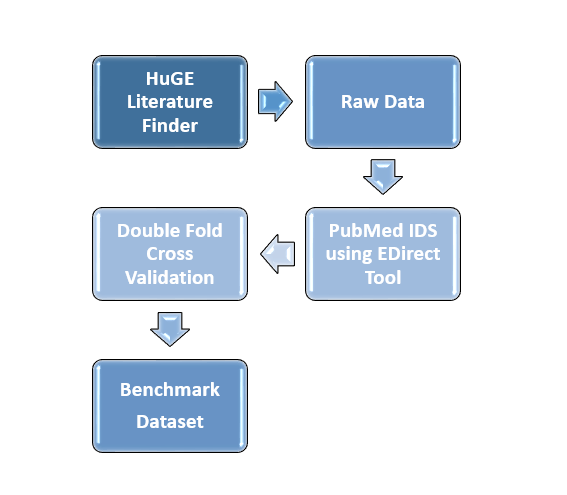
\includegraphics[width=0.8\linewidth]{Breast Cancer Flow.PNG}
    \caption{Process Flow Diagram}
    \label{fig:Process Flow BRCA1l}
\end{figure}









\chapter{Methodology}





\section{Work Flowchart }

\begin{figure}[!h]
    \centering
    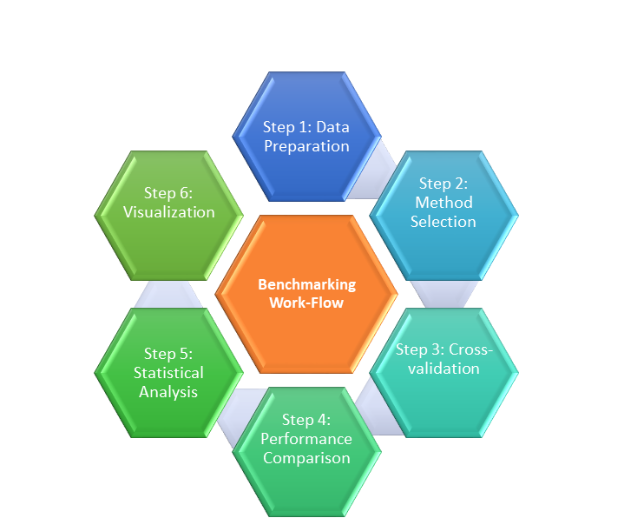
\includegraphics[width=0.8\linewidth,]{figures/methodology.png}
    \caption{Benchmarking Work-Flow}
   
    \label{fig:Benchmarking Work-Flow}
\end{figure}

\vspace{1cm}

Data preparation ensures data integrity through activities like removing duplicates, handling missing values, and structuring data.

Carefully select appropriate methodologies for the data and problem, considering data type, outcomes, and computational needs.

Cross-validation is a way to check how well a model performs on new data.This is done by dividing the data into multiple subsets. The model is then trained on one subset and evaluated on another. This process is repeated multiple times, each time using a different subset for training and evaluation.

Compare different methods using performance metrics like accuracy and precision to find the best approach for the task.

Use statistics to make sure the differences in method performance are real and not just random.

Show the results of the benchmarking using charts and graphs so everyone can understand them.


\section{Different ML Model Result}


Different machine learning models use various evaluation metrics to assess their performance on a given task. The choice of evaluation metric depends on the nature of the problem (classification, regression, clustering, etc.) and the specific goals of the model. 

\textbf{SVM (Support Vector Machine): }\newline
Accuracy: \textbf{60.41\%} SVM is a supervised machine learning algorithm used for classification and regression tasks. It works by finding the optimal hyperplane that best separates data points belonging to different classes. \newline
\textbf{RF (Random Forest):} \newline
Accuracy: \textbf{85.71\%} Random Forest is an ensemble learning method that operates by constructing a multitude of decision trees during training and outputting the class that is the mode of the classes (classification) or mean prediction (regression) of the individual trees. \newline
\textbf{DT (Decision Tree): }\newline
Accuracy:\textbf{ 72.91\%} A Decision Tree is a flowchart-like tree structure where an internal node represents a feature (or attribute), the branch represents a decision rule, and each leaf node represents the outcome. Decision trees are used for both classification and regression. \newline
\textbf{NN (Neural Network):} \newline
Accuracy:\textbf{80.65\%} (Note: "NN" is commonly used to represent Neural Networks) Neural Networks are a class of machine learning models inspired by the structure and functioning of the human brain. They consist of layers of interconnected nodes (neurons) and are capable of learning complex patterns. Neural Networks can be used for various tasks, including classification and regression. \newline

These accuracy values represent the performance of each model on a specific task or dataset. Higher accuracy generally indicates better performance, but it's essential to consider other metrics and factors depending on the specific requirements of your machine learning application. 


\begin{table}[!h]
    \centering
    \begin{tabular}{|c|c|} \hline 
         \textbf{Method Name}& \textbf{Accuracy}\\ \hline 
         Neural Network& 80.65\%
\\ \hline 
         SVM& 60.41\%
\\ \hline 
         Decision Tree
& 72.91\%
\\ \hline 
         Random Forest& 85.71\%
\\ \hline
    \end{tabular}
    \caption{Perfomance on Different Method}
    \label{tab:Evaluation Result}
\end{table}


 \begin{figure}[!h]
     \centering
     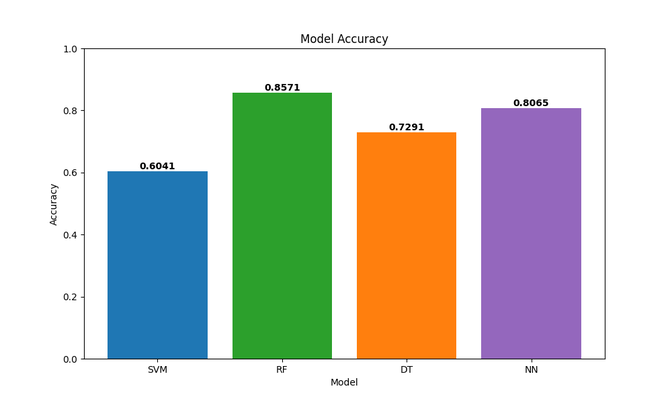
\includegraphics[width=1\linewidth]{Model Accuracy.png}
     \caption{Accuracy Perfomance Histogram}
     \label{fig: Accuracy Histogram}
 \end{figure}

From the study above, it is clearly seen that the Random Forest gives the best accuracy on the dataset of breast cancer. \cite{33}

\chapter{Future Work and Conclusion}

\section{Conclusion}


The thesis has undertaken a comprehensive exploration of a wide spectrum of genes responsible for causing diseases that adversely impact human well-being. This investigation involved a thorough and meticulous examination of the intricate genetic factors contributing to various ailments. By delving into the underlying genetic mechanisms, the thesis has illuminated the complex web of factors that give rise to these diseases.

One significant outcome of this in-depth analysis is the identification of potential avenues for further research. The revelations made in the thesis provide a solid foundation for scientists and researchers to delve deeper into the molecular and genetic intricacies of these diseases. This, in turn, opens up new possibilities for uncovering novel insights that may have been previously overlooked.

Moreover, the thesis serves as a catalyst for the development of precise therapeutic strategies. Armed with a deeper understanding of the genetic basis of diseases, researchers and medical professionals can now work towards the design and implementation of targeted and effective treatment approaches. This precision in therapeutic strategies holds great promise for improving patient outcomes, minimizing side effects, and ultimately enhancing the overall efficacy of medical interventions.

In essence, the thesis not only contributes to our understanding of the genetic roots of diseases but also serves as a springboard for future scientific inquiries. It lays the groundwork for advancements in medical research and the development of innovative treatments that have the potential to alleviate the burden of various ailments on human health and well-being.

\section{Future Work:}

Our future research endeavors will be directed towards the advancement of a benchmark dataset by integrating multi-omics data, temporal information, and validation on larger datasets. With a particular emphasis on interpretability and visualization, we aim to facilitate the acquisition of clearer insights into human disease genes. The enriched dataset will subsequently be applied to the field of precision medicine, enabling the development of personalized and targeted treatments, ultimately leading to improved patient outcomes.

As the field of machine learning continues to evolve, several exciting avenues for future research emerge, focusing specifically on NNs, SVMs, decision trees, and RFs:

1. Hybrid Models: Combining different machine learning algorithms, such as NN-SVM or RF-decision tree ensembles, can potentially enhance performance by leveraging the strengths of each approach.

2. Feature Selection: Identifying the most relevant and informative features from the vast amount of biological data can improve the predictive accuracy of machine learning models.

3. Model Optimization: Developing efficient algorithms for parameter tuning and training of complex models, particularly NNs, can reduce computational complexity and improve scalability.

4. Explainability and Interpretability: Increasing the understanding of how machine learning models make predictions, particularly for complex models like NNs, is crucial for gaining trust and ensuring responsible use in gene-disease association prediction.

5. Clinical Applications: Translating machine learning predictions into actionable clinical insights and developing real-time applications can revolutionize personalized medicine and improve patient outcomes.

By addressing these challenges and exploring these promising directions, machine learning has the potential to revolutionize our understanding of gene-disease associations and transform the future of healthcare.
